

\documentclass[12pt,oneside,english]{article}

%\usepackage[T1]{fontenc}
\usepackage[latin1]{inputenc}
\usepackage{geometry}
\geometry{verbose,letterpaper,tmargin=1in,bmargin=1in,lmargin=1in,rmargin=1in}
\usepackage{textcomp}
\usepackage{babel}
\setcounter{secnumdepth}{3}
\usepackage{graphicx}
\usepackage{float}
\floatstyle{boxed}
\restylefloat{figure}
\usepackage{longtable}
\usepackage{url}

\usepackage{listings}
\usepackage{color}

\definecolor{mygray}{rgb}{0.4,0.4,0.4}
\definecolor{mygreen}{rgb}{0,0.8,0.6}
\definecolor{myorange}{rgb}{1.0,0.4,0}

% \lstset{language=Matlab,
%    keywords={break,case,catch,continue,else,elseif,end,for,function,
%       global,if,otherwise,persistent,return,switch,try,while},
%    basicstyle=\sffamily,
%    keywordstyle=\color{blue},
%    commentstyle=\color{dkgreen},
%    stringstyle=\color{red},
%    numbers=left,
%    numberstyle=\tiny\color{gray},
%    stepnumber=1,
%    backgroundcolor=\color{white},
%    tabsize=4,
%    showspaces=false,
%    showstringspaces=false}
% \lstset{
% basicstyle=\footnotesize\sffamily\color{black},
% commentstyle=\color{mygray},
% frame=single,
% numbers=left,
% numbersep=5pt,
% numberstyle=\tiny\color{mygray},
% keywordstyle=\color{mygreen},
% showspaces=false,
% showstringspaces=false,
% stringstyle=\color{myorange},
% tabsize=4
% }

\newcommand{\BibTeX}{{\sc Bib}\TeX}


\begin{document}



% Thesis Lessons %
\section{Thesis Lessons}

This paper also illustrates how a high knowledge uncertainty in the independant variable (temperature) can skew experiment conclusions.  
The knowledge uncertainty in temperature is quantified by using bare (non nanoisland-producing) sample measurements; 
    multiple thermocouple measurements revealed temperature gradients across the oven.
During rapid heating, the measured oven temperature is generally skewed higher than the sample temperature.

% Thesis as designed %
\section{Thesis as designed}

This thesis was started with the goal of producing repeatable nanoisland morphology; 
the size and shape of nanoislands produced through self-assembly, thermolysis, and annealing would be characterized through atomic force microscope measurements.

Because the nanoislands previously measured have been elliptical in shape, these nanoisland sizes can be characterized by area or by equivalent diameter, 
where equivalent diameter is related to area using a circular approximation (Equation ~\ref{eq:equiv_diameter}).
\begin{equation}
    d = \sqrt{ A \cdot 4 \over{\pi} }
\label{eq:equiv_diameter}
\end{equation}

In this thesis plan, the distribution of shapes of these nanoislands would be evaluated by the analyst.
Since previous results indicated that roughly elliptical islands would be formed, the semi-major and semi-minor axes could be measured, along with the orientation of the semi-major axis.  
Characterization of the equivalent ellipse can be automated by "blob finder" algorithms, by Matlab, and by Gwyddion Grain Analysis scripts.  
When nano-islands could not be measured during this thesis due to equipment failure, the computer-vision and automated measurement components developed for this thesis plan were used to evaluate archival nanoisland images.

[reference: http://gwyddion.net/documentation/user-guide-en/grain-analysis.html]

Also in this plan, the effect of variations in size, shape, and orientation was to be evaluated by the absorption features. 
The absorption features of interest are caused by surface plasmon resonance of the nanoislands.

[reference definitely needed for definitive statement: absorption features <- surface plasmon resonance]

This absorption feature is shown (shon plasmonics proof) before and after protein binding, where the protein was used as a receptor for a particular atmospheric contaminant.

[Insert figures from etched plasmonics proof -- Figures 6 and 9 show some spectra before and after various stages of bonding/binding.]

By quantifying the distribution of size, eccentricity, and orientation of the islands, 
and by quantifying the strength and breadth of the absorption spectrum, 
correlations may be found to indicate whether self-assembly is sufficient to produce repeatable samples using a largely-manual laboratory process.

The thesis as run significantly deviated from this concept due to the unavailability of the atomic force microscope necessary to characterize the samples.  
The loss of the AFM meant spectroscopy of the samples could not be correlated against size and shape statistics.

% section break %
% Thesis as run %
\section{Thesis as run}

This thesis, as run, looks at in-situ impedance and thermocouple temperature measurements during sample creation, and sets forth procedures for creating, annealing, and analyzing nanoisland samples.  
Where possible, simple automation was introduced to facilitate the acquisition of data and the accurate measurement of temperature.
Automation was also created to calculate statistics of nano-island images.

% The next paragraph makes the distinction between "temperature" (which implies "sample temperature") and "thermocouple temperature".  %
% We do not measure the sample temperature. %
Automation was introduced to slow down oven heating, and facilitated the automated collection of temperature measurements.
Thermocouple temperature measurements were collected at 1Hz sampling, in conjunction with the in-situ sample impedance measurements 
    during heating, thermolysis, and annealing.  
To quantify the accuracy of thermocouple measurments in predicting sample temperature, 
    impedance was also measured for bare test samples on which no material had been deposited. 

It was expected that the sample impedance at a given thermocouple temperature measured during fast heating should match the impedence at the same thermocouple temperature measured during slow cooling.
Discrepancies in impedance vs. temperature, between fast heating and slow cooling, show accuracy uncertainty in the thermocouple measurement as a predictor of sample temperature.

%% MOTIVATION: Use the UKC Abstract 2012 for the background material. %%
%%     SEE: UKC ABSTRACT AT END OF DOCUMENT. %%
\section{Motivation: Measurements during nano-island formation}

The motivation for this thesis came from an observation of in-situ impedance during fast heating and annealing of self-assembled Au$_{314}$ multi-layer film.
This measurement suggested that the thermolysis process during self-assembly and annealing contained a measured phase change in which impedance dropped, 
    in which a contiguous path across the gold nano-island precursors might have formed, before the film separated into islands.
This sequence of events did not recur in other samples measured in-situ, nor did it recur in this thesis.

Gold nano-islands are very sensitive to any plasmon changes on their surface boundary, offering chemical and bio-sensing applications.
Polymer-mediated self-assembly is a low-cost alternative to evaporation or sputtering for depositing gold on a substrate [1,2].  Gold nanoparticles may be functionalized by organic molecules and deposited layer by layer using self-assembly to create layers predictably.
Nano-islands are formed from these layers by thermolysis of the organic molecules at high temperatures, and subsequently annealing the resulting gold film at a temperature between 600$^{\circ}$C to 650$^{\circ}$C.

In the prior thesis work, and in this thesis, a pre-patterned inter-digitated electrode (IDE) glass substrate was dipped in a solution of Au$_{314}$ nanoparticles functionalized with organic ligands to form a monolayer.  
The functionalized ligands bond to the substrate in a single layer.
Activation of the first layer with poly(allyl amine) hydrochloride (PAH) allows the next layer to be deposited by a second dipping.  
The process is repeated until 8 layers are deposited.

Figure: Resistance versus temperature is plotted for a multilayer sample (black) and for a bare IDE (blue).  The arrows indicate the direction of the temperature changes during the measurement.

The sample impedance was measured in situ during the high temperature heating and cooling by a four-point measurement at 1kHz frequency.
Compared to the bare IDE substrate, the self-assembled gold sample showed several distinct features while heating.
The most notable feature was a sharp decrease in impedance at 560$^{\circ}$C, reaching less than 100 $\Omega$ at 570$^{\circ}$C.
Above 620$^{\circ}$C the resistance increased sharply. 

The sharp decrease in resistance around 560$^{\circ}$C suggested the structural integrity of polymers is compromised and the gold nano-particles start forming a conductive percolative network or that a short circuit path was formed between two digits of the IDE.
The increased resistance at 625$^{\circ}$C indicates the formation of nano-islands through the aggregation and the embedding of nano-islands on the glass.

Prior work has used variations in which more or fewer layers are deposited, in which alternate materials are substituted for Au$_{314}$, 
    and in which layers alternate between two materials (silver and gold).

%% THEORY OF IMPEDENCE OF SEMI-INSULATING MATERIALS %%
\section{Theory of Impedance of Semi-Insulating Materials}
Impedance measurements follow a temperature dependence derived from models of electron transport under an AC potential.  
Frequency and temperature dependance follows for non-surface-effect conductance.
Complex impedance and temperature measurements are used to solve electron mobility under the AC electron transport model.

    \subsection{Electron Transport Measurement using Complex Impedance}
    Impedance measurements follow a temperature dependence derived from models of electron transport under an AC potential [citation needed].  
    
    \begin{equation}
        R = R_0 \cdot e^{\epsilon\over{k \cdot T}}
        \label{eq:emobility}
    \end{equation}
    
    This equation can be rearranged into a linear equation to solve for $\epsilon$.
    
    \begin{equation}
        ln(R) = {\epsilon\over{k}} {1\over{T}} - ln(R_0)
        \label{eq:solve_emobility}
    \end{equation}
    
    ${\epsilon\over{k}}$ and $ln(R_0$ are found by least-squared fit of the linear portion of the data.
    
    The resistance $R_p$ of a high-resistance sample can be measured from the complex impedance $(Z,\theta)$ by Equation ~\ref{eq:R_p}.  Use of the parallel resistance $R_p$ is justified at high sample resistance because the series resistance $R_s$ of the test leads and contacts are orders of magnitude smaller.
    
    \begin{equation}
        R_p = {{Z} \over {cos({\theta})}}
        \label{eq:R_p}
    \end{equation}

    \subsection{Experimental Impedance Characterization Procedure}

    \begin{figure}
    
    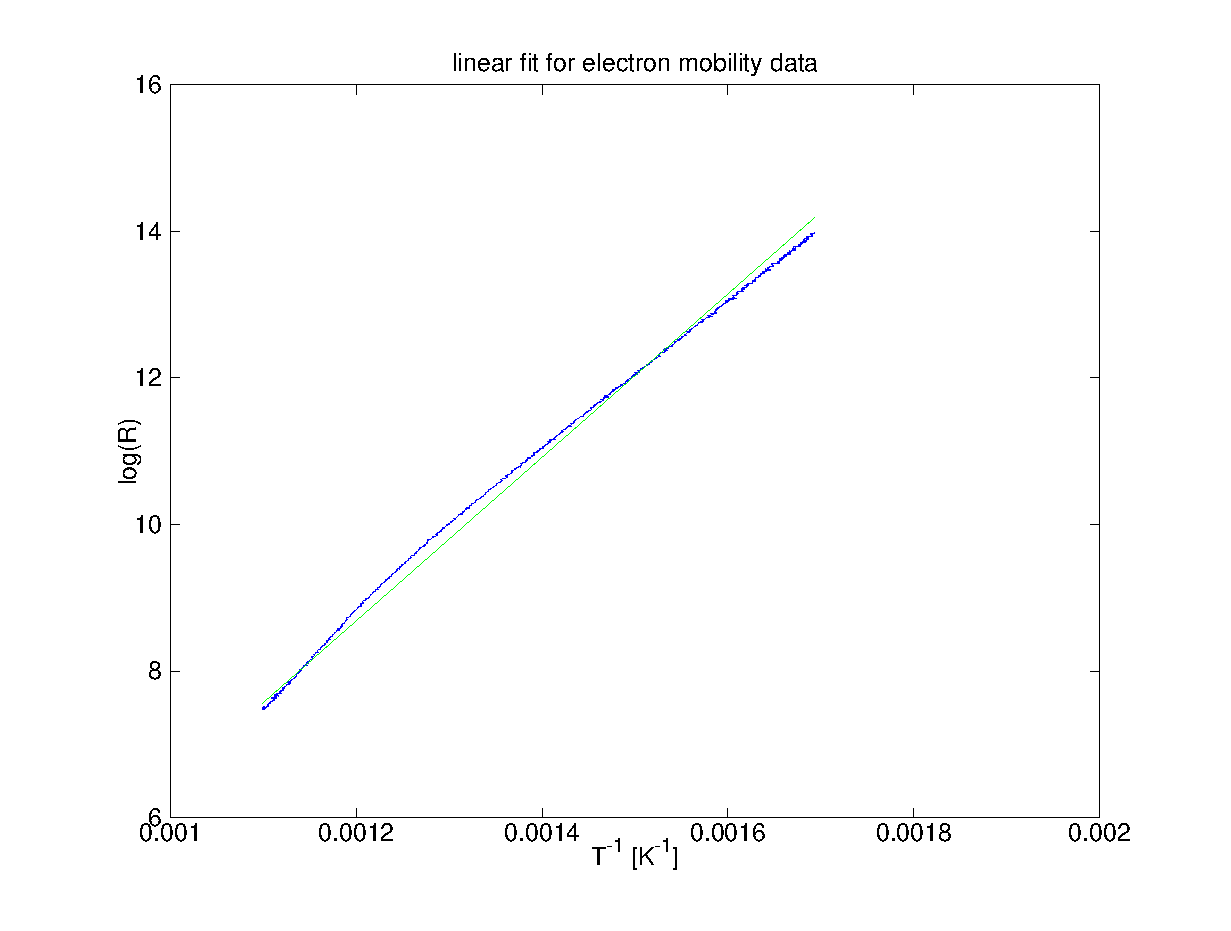
\includegraphics[scale=0.4]{images/electron_mobility.eps} 
    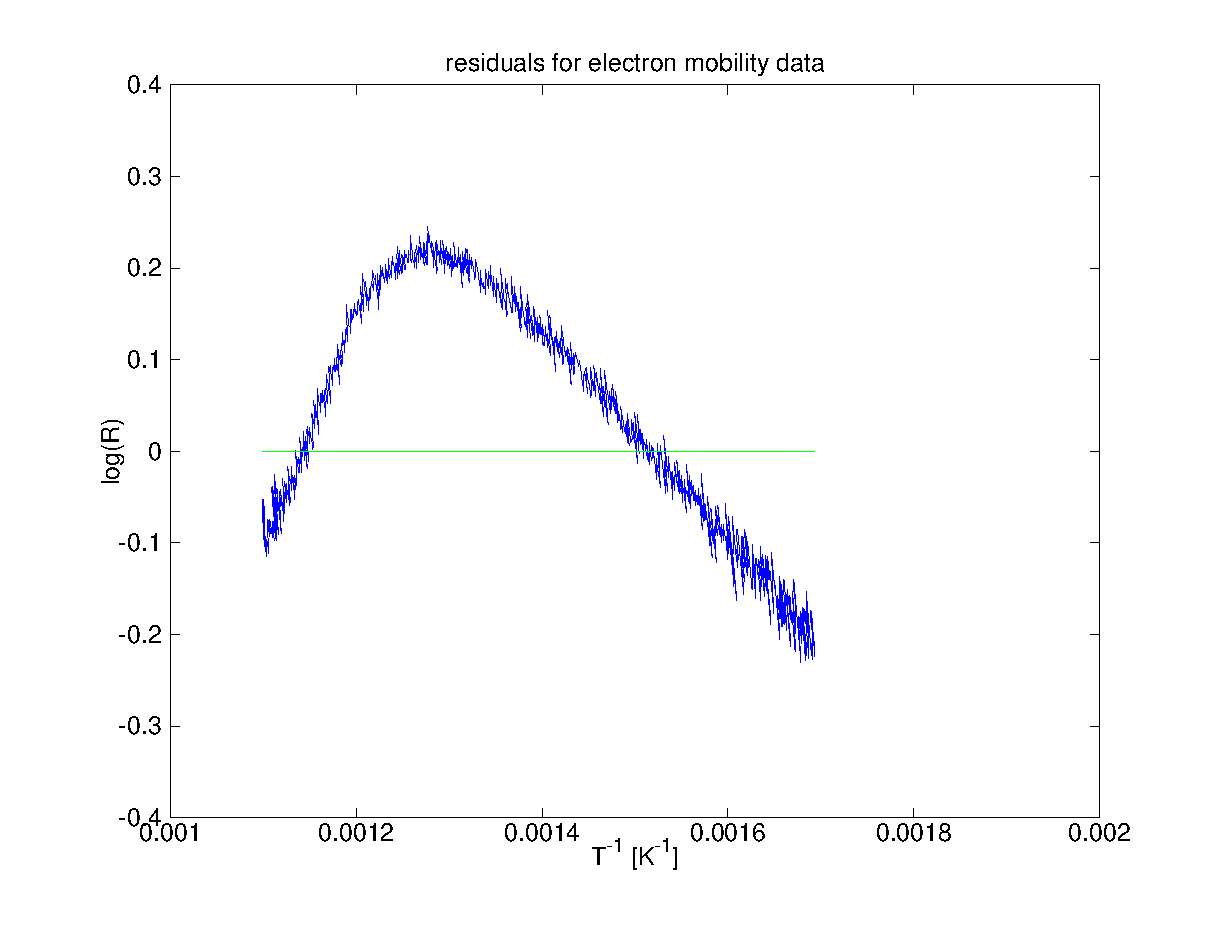
\includegraphics[scale=0.4]{images/electron_mobility_residual.eps}
    \label{f:emobility}
    \caption{During cool-down of the sample, the impedance versus temperature measurements are well-sampled, and can be used to solve for electron mobility.  ${\epsilon\over{k}} = 1.1e+04 K$, $\epsilon = 0.96 eV$, $R_0 = 9.1e-3\Omega$.  Error bars are needed, and will have magnitude at least proportional to the fit residuals.  The curve in the logarithmic plot indicates an uncompetnsated offset bias.}
    \end{figure}

    Impedance of the IDE sample (device under test, or DUT) was measured as a complex number, using an Agilent 82XX LCR meter.
    Temperature measurements were limited to those measurements taken during cool-down of the DUT, since temperature measurements during fast heating of the sample carry very large errors.  
    Measurements of impedance over temperature during cool-down (FIGURE "cooldown\_residuals") were identical within uncertainties for the Au$_{25}$ sample (JD04) and a bare IDE sample (JD05), and electron mobility will be identical.  
    Electron mobility calculated for the Au$_25$ (JD04) sample was ${\epsilon\over{k}} = 1.1e+04 K$, $\epsilon = 0.96 eV$.
    DC resistance measurements of the electrode show only its insulating properties, as the glass substrate is a poor conductor and the IDE is a weak capacitor, so AC resistance is measured.
    AC resistance in the IDE samples follows the temperature-dependent electron mobility.

    The temperature range observed is between $295K$ and $900K$, 
    
    Sample resistance (a parallel AC resistance) is typically high for the sample under test, this resistance changes when the sample is heated and the polymers are burned off.  

    
    Typical values for complex impedance measured by the auto-balancing bridge method via an Agilent 82XX LCR meter are as follows.
    
    \begin{equation}
        \left( Z,\theta,\nu,T \right) = \left( 15 M\Omega, -89.9^\circ, 1kHz, 22^{\circ}C \right)
    \end{equation}
    \begin{equation}
        \left( Z, \theta, \nu, T \right) = \left( 800 k\Omega, -88^\circ, 45kHz, 22^{\circ}C \right)
    \end{equation}
    
    This result shows that the $R_p$ ``resistance'' component (which is $Z$ divided by $cos(-89^\circ)$) is immeasurably high at low frequencies and low temperature.  It is only at higher temperatures that $R_p$ drops to the measurable range, and this occurs at about $250^{\circ}C$ when the impedance phase angle $\theta$ drops from $-89.9^\circ$ towards $0.1^\circ$.
    
    During the burn-off of the polymers, the parallel resistance may drop to under 100 ohms, which requires a four-point measurement to compensate for the series resistance test lead impedance.
    A four-point measurement is necessary because the test leads have been reported (AD5933) to have up to kilo-ohm impedance when measuring low sample resistance.




%% PROCEDURE %%

\input{mark_end.tex}


----------------------------------------------------------------------------
From UKC Abstract: 
"In-situ Impedance Measurement Of Gold Nano-Island Self-Assembly Shows Chemical 
    and Structural Changes During Heating and Annealing"

REFERENCES
1.     Shon, Bull. Korean Chem. Soc. 2010, Vol. 31, No. 2 291.
2.    Shon, Kwon. J. Phys. Chem. C, 2011, 115 (21), pp 10597–10605
----------------------------------------------------------------------------

A = pi * r^2 = pi * d^2 / 4
d = sqrt { A / pi * 4 }
